\chapter{Test utilisateurs}
	Le test utilisateur est une étape indispensable pour valider les
	théories développées durant le travail de recherche et conception.
	Ces tests auront pour but de valider deux aspects du framework : Ses
	performances lords de la peinture d'image gigapixel, et la qualité
	de son anti-aliasing. 

	\section{Procédure}
		Le but de la procédure est d'arriver à obtenir de l'artiste une
		information fiable sur la performance du framework et la qualité du rendu. 
		Cela n'est pas une chose évidente puisque l'artiste ne fait habituellement
		pas la différence entre l'interface utilisateur et le framework utilisé pour
		le rendu. 

		\subsection{Premiers tests}
		En effet, les premiers tests furent réalisés avec une interface graphique fort
		austère et différente des logiciels que les artistes avaient l'habitude d'utiliser.
		La pluspart de leurs critiques étaient centrées sur l'interface utilisateur, et
		leur évaluation des performances semblaient affectées par la frustration générée
		par l'interface graphique.

		Nous avons donc décidé d'améliorer l'interface en répondant aux principales critiques
		des utilisateurs:
		\begin{itemize}
			\item nécessité d'avoir un outil permettant de sélectionner une couleur à l'écran.
			\item nécessité d'avoir des raccourcis clavier similaires à \emph{Adobe Photoshop}
			\item nécessité d'avoir une visualisation de la taille de la brush autour du curseur.
		\end{itemize}

		\begin{figure}[ht]
			\centering
			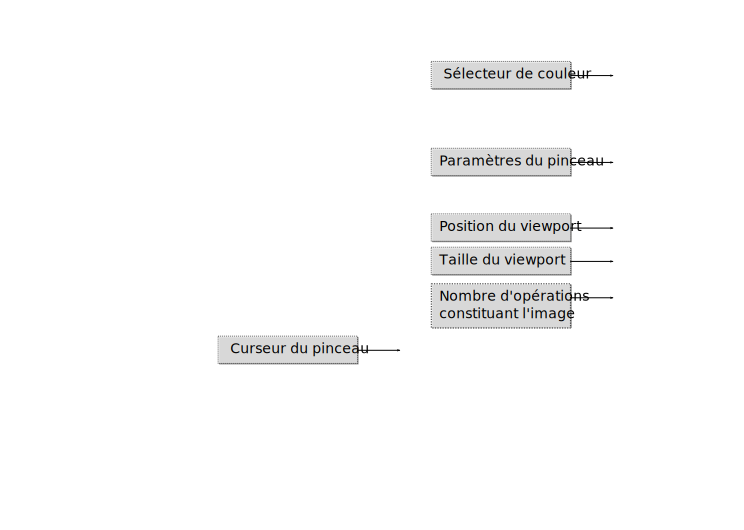
\includegraphics[width=\textwidth]{images/screenshot} 
			\caption{Screenshot de l'application utilisée pour les tests utilisateurs}
			\label{fig:screenshot}
		\end{figure}
		Ces fonctionalités furent donc implémentées, et les tests refaits. Un screenshot de l'application
		de test se trouve à la figure~\ref{fig:screenshot}, page~\pageref{fig:screenshot} 

		\subsection{Second tests}
			\subsubsection{Matériel utilisé}
			Afin de rendre comparable les évaluations de performances avec les discussions des
			précédent chapitres, les tests utilisateurs ont été réalisés sur la machine de développement.
			Il s'agit d'un ordinateur portable avec un processeur intel à deux cores à 1.66Ghz, disposant
			de 2Go de RAM, d'un écran 1024x768, avec le système d'exploitation Linux Debian Lenny.

			Les utilisateurs avaient également à leur disposition une tablette graphique Wacom Bamboo.

			\subsubsection{Première étape}
			Nous commencons par une démonstration exhaustive des fonctionalités du programme.
			Ensuite nous expliquons le but de l'expérience; l'évaluation de la fluidité de
			l'édition, et la qualité de l'anti-aliasing --- et non pas de l'interface utilisateur.
			Nous terminons cette première étape par énoncer et expliquer toutes les étapes qui vont suivre,
			afin que l'utilisateur ne soit pas pris au dépourvu à chaque étape.

			\subsubsection{Second étape}
			Cette seconde étape constitue en une familiarisation avec l'interface. L'utilisateur
			a pour consigne de prendre le temps qu'il désire pour se familiariser avec le programme
			et tester ses fonctionalités. 

			\subsubsection{Troisième étape}
			Les performances et la qualité du rendu peut dépendre du type de dessin réalisé. Ainsi
			nous allons explorer dans cette étape un des deux grands styles de dessin, le dessin au trait.
			Il est donc demandé à l'utilisateur de réaliser un portrait au trait, en noir et blanc de préférence.
			Il dispose pour cela d'une durée de vingt minutes. 


			L'utilisateur commence avec une feuille de dessin blanche de $800 \times 600$ Millions de pixel, au cinquième
			niveau de zoom, ce qui représente une zone par défaut d'un demi gigapixel. 

			Pendant cet étape, l'évaluateur observe, note les commentaires de l'utilisateur, et répond aux questions
			éventuelles. 

			On notera que la durée des tests, vingt minutes, est assez courte. Elle ne permet pas toujours au testeur
			de terminer son dessin. Cette durée est intensionellement limitée pour ne pas demander trop de temps aux testeurs
			bénévoles, mais aussi pour éviter d'atteindre la limite de mémoire de la machine, étant donné que 
			le programme ne dispose pas encore de mécanisme global permettant de limiter son usage. 

			\subsubsection{Quatrième étape}
			Cette étape impose le deuxième style, la peinture à l'applat. Il est donc demandé à l'utilisateur de
			réaliser un portrait en couleur en utilisant des techniques de peinture. 
			Il dispose pour cela d'une durée de vingt minutes. 

			L'utilisateur commence avec une feuille de dessin blanche de $800 \times 600$ Millions de pixel, au cinquième
			niveau de zoom, ce qui représente une zone par défaut d'un demi gigapixel. 

			Pendant cet étape, l'évaluateur observe, note les commentaires de l'utilisateur, et répond aux questions
			éventuelles. 

			\subsubsection{Cinquième étape}
			Cette dernière étape est conçue pour forcer les utilisateurs à utiliser toute la résolution d'une image
			gigapixel. Pour cela nous leur demandons de dessiner dans la technique de leur choix \emph{Un homme sur
			un éléphant, avec dans sa poche une puce} Le tout en respectant les échelles. 

			L'utilisateur commence avec une feuille de dessin blanche de $800 \times 600$ Millions de pixel, au sixième
			niveau de zoom, ce qui représente une zone par défaut de deux gigapixels

			Pendant cet étape, l'évaluateur observe, note les commentaires de l'utilisateur, et répond aux questions
			éventuelles. 

			\subsubsection{Évaluation}
			Après chaque étape nécessitant une interaction avec le programme, il est demandé à l'utilisateur de donner
			une note entre un et cinq sur les points suivants:
			\begin{itemize}
				\item Les performances lors de la peinture
				\item Les performances lors du déplacement de la région visualisée.
				\item Les performances lors du zoom/dezoom
				\item La qualité de l'anti-aliasing
			\end{itemize}
			Les notes étant expliquées de la manière suivante:
			\begin{enumerate}
				\item[1] inacceptable.
				\item[2] mauvais.
				\item[3] correct.
				\item[4] bien.
				\item[5] excellent.
			\end{enumerate}
			Et ceci en comparaison avec les logiciels qu'ils ont l'habitude d'utiliser dans le cadre de leur travail. 
	\section{Résultats}
		L'application fut testée par trois artistes :
		\begin{description}
			\item[Brice Vandemoortele] Travaille en tant que texture-artist indépendant dans l'industrie du jeu-vidéo. Il est également
			expert auprès de la Commission d'Art Numérique de la Communauté Française de Belgique. 
			\item[Jean-François Brogniet] Est matte-painter dans l'industrie de l'animation en images de synthèse.
			\item[Jean-Philippe Servais] Est matte-painter et concept designer dans l'industrie de l'animation en images de synthèse. 
		\end{description}
		
		Lors des tests furent enregistrées toutes les actions entreprises par les artistes. Les performances du programme lors du test ont également
		été enregistrées. Ceci afin de pouvoir comparer de manière quantitative l'avis des artistes et les performances telles qu'ils les
		ont expérimentées. Ces enregistrement pouvant être rejoués, il serait possible d'évaluer l'influence des modifications du framework sur
		les performances dans des cas d'utilisation réelle. 

	\begin{table*}
		\small
		\begin{tabular*}{\textwidth}{@{\extracolsep{\fill}} | l || c | c | c | c | c || c | c | c | c | c | }
		\hline
					&\multicolumn{5}{c||}{Performances}						&\multicolumn{5}{c|}{Avis}\\
		\hline
		Utilisateur		& \sw{Mean RT}	& \sw{Max RT}	& \sw{Median SL}&\sw{Max SL}	&\sw{SL Count}	& \sw{Peinture}	& \sw{Pan}	& \sw{Zoom} 	& \sw{U/R}	& \sw{AA}	\\
		\hline
		\multicolumn{11}{l}{Test 1: Familiarisation avec l'interface}\\
		\hline
		Brice			& 0.012		& 1.21		& 0.19		& 13.55		& 567		& 5		& 5		& / 		& 5		& /	\\	
		Jean-Philippe		& 0.013		& 1.56		& 0.15		& 2.25		& 225 		& 4 		& 3		& 3		& 4		& 5 	\\
		Jean-François		& 0.024		& 3.91		& 0.20		& 10.6		& 830 		& 3		& 4		& 2		& 4		& 5	\\
		\hline
		\multicolumn{11}{l}{Test 2: Dessin d'un portrait au trait}\\
		\hline

		Brice			& 0.013		& 8.00		& 0.39		& 18.9		& 510		& 5		& 4		& 2 		& 5 		& 2	\\	
		Jean-Philippe		& 0.011		& 0.46		& 0.29		& 50.91		& 652 		& 3*		& 4		& /		& 2*		& 4 	\\
		Jean-François		& 0.029		& 11.89		& 0.16		& 7.46		& 654 		& 3		& 3		& 1		& 4 		& 3*	\\

		\hline
		\multicolumn{11}{l}{Test 3: Peinture d'un portrait}\\
		\hline
		Brice			& 0.017		& 8.67		& 0.17		& 15.73		& 1007		& 5		& 4		& 2 		& 5 		& 3	\\	
		Jean-Philippe		& 0.020		& 5.9 		& 0.16		& 3.29		& 703 		& 4 		& 4		& 2		& 2*		& 4 	\\
		Jean-François		& 0.023		& 4.37		& 0.20		& 4.85		& 1405 		& 3		& 3		& 1		& 4 		& 4*	\\
		\hline
		\multicolumn{11}{l}{Test 4: Peinture d'un homme et d'une puce sur un éléphant}\\
		\hline
		Brice			& 0.027		& 38.68		& 0.20		& 24.84		& 974		& 5		& 3		& 2 		& 3 		& 3	\\	
		Jean-Philippe		& 0.029		& 2.99		& 0.31		& 4.88		& 500 		& 4 		& 3		& 2		& 2*		& 5 	\\
		Jean-François		& 0.021		& 3.55		& 0.16		& 2.93		& 1267 		& 3		& 3		& 1		& 4 		& 4*	\\
		\hline
		
		\end{tabular*}
		\label{comparaison}
	\end{table*}


		
		également enregistré les performances du
		programme.
		

		
		
	\section{Analyse}
\chapter{Conclusion}
